
\section{\trRiemann--\trHurwitz{}公式}

\trRiemann--\trHurwitz{}公式将我们对 $\mathbb{P}^1$ 的那个在 $2g+2$ 个点处\trRamification{}的\trDoubleCover{}所算得的\trGenus{} $g$（\mbox{定理~19.5.1}）推广到了更高次数的覆盖，以及\trGenus{}更高的目标曲线。

\textbf{21.4.1.}\ \emph{\trhDefinition{}。}\quad 称整\trScheme{}之间的一个有限态射 $X\to Y$ 为\textbf{\trSeparable}的（separable），若它是\trDominant{}的，且其诱导的函数域扩张 $K(X)/K(Y)$ 是一个可分扩张。类似地，称一个\trGenericallyFinite{}态射为\textbf{\trGenericallySeparable}的（generically separable），若它是\trDominant{}的，且其诱导的函数域扩张是一个（有限）可分扩张。注意，在\trCharacteristic{} $0$ 时，整\trScheme{}之间的有限态射自动可分。

\textbf{21.4.2.\ \trhProposition。}\ ——\ \emph{设 $\pi\colon X\to Y$ 是同维数 $n$ 的不可约\trVariety{}之间的一个\trGenericallySeparable{}\trMorphism，且 $Y$ 光滑。那么余切正合列（\mbox{定理~21.2.24}）也\trLeftExact{}：}
\begin{equation*}\tag{21.4.2.1}\label{eq:cotangent-left-exact}
0\longrightarrow\pi^*\Omega_{Y/k}\xrightarrow{\ \phi\ }\Omega_{X/k}\longrightarrow\Omega_{X/Y}\longrightarrow 0.
\end{equation*}

这是余切正合列在适当「光滑性」之下\trLeftExactness{}的一个例子；见\mbox{注记~21.2.10}。

\emph{证明。}\quad 我们必须检验 $\phi$ 是单射。$\Omega_{Y/k}$ 是 $Y$ 上秩 $n$ 的\trLocallyFreeSheaf，所以 $\pi^*\Omega_{Y/k}$ 是 $X$ 上秩 $n$ 的\trLocallyFreeSheaf。整概形上的\trLocallyFreeSheaf（比如 $\pi^*\Omega_{Y/k}$）是无挠的（任一开集上的非零\trSection{}在\trGenericPoint{}处非零；见 \S6.1.4），所以若它的一个子层（比如 $\ker\phi$）非零，它便在\trGenericPoint{}处非零。于是要证 $\phi$ 的单性，只须检验 $\phi$ 在\trGenericPoint{}处是一个含入映射。我们从而以 $\OO_\eta$ 作张量，其中 $\eta$ 是 $X$ 的\trGenericPoint。以 $\OO_\eta$ 作张量是一个正合函子（局部化正合，\mbox{练习~1.5.G}），而 $\OO_\eta\otimes\Omega_{X/Y}=0$（因为按假设 $K(X)/K(Y)$ 是可分扩张，而可分域扩张的 $\Omega$ 为 $0$，见\mbox{练习~21.2.H(a)}）。此外，$\OO_\eta\otimes\pi^*\Omega_{Y/k}$ 与 $\OO_\eta\otimes\Omega_{X/k}$ 都是 $n$ 维的 $\OO_\eta$-\trVectorSpace（它们是秩 $n$ 的\trLocallyFreeSheaf{}在\trGenericPoint{}处的茎）。于是考虑
\[
\OO_\eta\otimes\pi^*\Omega_{Y/k}\longrightarrow\OO_\eta\otimes\Omega_{X/k}\longrightarrow\OO_\eta\otimes\Omega_{X/Y}\longrightarrow 0
\]
（即 $\OO_\eta^{\oplus n}\to\OO_\eta^{\oplus n}\to 0\to 0$），我们便看出 $\OO_\eta\otimes\pi^*\Omega_{Y/k}\to\OO_\eta\otimes\Omega_{X/k}$ 是单射，从而 $\pi^*\Omega_{Y/k}\to\Omega_{X/k}$ 是单射。\hfill$\square$

不局限于\trCharacteristic{} $0$ 的人应当留意：对非\trSeparable{}的\trMorphism{}而言，事情会怎样出岔子。例如，设 $k$ 是\trCharacteristic{} $p$ 的域，考虑由 $u=t^p$ 给出的\trMap{} $\pi\colon\mathbb{A}^1_k=\Spec k[t]\to\mathbb{A}^1_k=\Spec k[u]$。此时 $\Omega_\pi$ 是由 $\mathrm{d}t$ 生成的平凡\trInvertibleSheaf。再举一个（相似但不同的）例子：若 $K=k(x)$、$K'=k(x^p)$，则含入映射 $K'\hookrightarrow K$ 诱导 $\pi\colon\Spec K[t]\to\Spec K'[t]$。此时 $\Omega_\pi$ 仍是一个\trInvertibleSheaf，由 $\mathrm{d}x$ 生成（而 $\mathrm{d}x$ 在此情形是从 $\Spec K$ 上的 $\Omega_{K/K'}$ 拉回的）。在这两个例子中，我们都有一条仿射直线到另一条仿射直线的\trMap，并且存在非零的相对\trTangentVector。

\textbf{21.4.A.（练习）}\quad 设 $X$ 与 $Y$ 都是维数 $n$ 的光滑\trVariety，而 $\pi\colon X\to Y$ \trGenericallySeparable。证明：非光滑性轨迹是纯余维数 $1$ 的，并且（如下所述）有一个作为有效除子的自然诠释。在适当的局部坐标下，把 $\phi$ 诠释为一个 $n\times n$ \trJacobianMatrix{} \eqref{eq:jacobian-corank-matrix}，从而把 $\phi$ 非同构的轨迹诠释为（局部地）某个 $n\times n$ 矩阵的行列式的消失概形。

我们把非光滑性轨迹（在 $X$ 中的）称作\textbf{\trRamificationLocus}（ramification locus），而把它在 $Y$ 中的像称作\textbf{\trBranchLocus}（branch locus）。正是因为这道练习，我们才使用\textbf{\trRamificationDivisor}（ramification divisor）以及（假设\trRamificationDivisor{}的像确实是一个除子）\textbf{\trBranchDivisor}（branch divisor）这两个术语。

在着手处理我们感兴趣的维数 $1$ 情形之前，我们先来做一件（名副其实）小但有趣的事。设 $\pi\colon X\to Y$ 是从光滑 $k$-概形出发的一个满 $k$-态射，它把一个余维数大于 $1$ 的子集收缩掉。更精确地说，设 $\pi$ 限制在 $X$ 的一个开子集 $\mathrm{U}$ 上是到 $Y$ 的某个开子集上的同构，而 $\mathrm{U}$ 的余集余维数大于 $1$。那么由\mbox{练习~21.4.A}，$Y$ \emph{不可能}光滑。（\emph{\trSmallResolution}（small resolutions，将于\mbox{练习~22.4.N}中定义）就是这类 $\pi$ 的例子。特别地，你可以在那里找到一个例子。）

现在设 $X$ 与 $Y$ 的维数为 $1$。那么\trRamificationLocus{}是 $X$ 的一个有限集（\textbf{\trRamification{}点}（ramification points）），而\trBranchLocus{}是 $Y$ 的一个有限集（\textbf{\trBranchPoint}（branch points））。（\cref{fig:branch-divisor-multiplicity} 展示了一个带两个分歧点与一个分支点的\trMorphism。）\emph{现在假设 $k=\bar{k}$。}我们在一点 $p\in X$ 附近考察 $\Omega_{X/Y}$。

\begin{figure}[htbp]
\centering
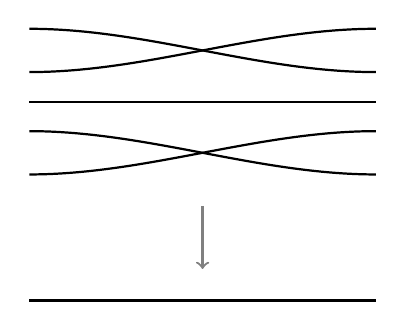
\begin{tikzpicture}[scale=1,line width=0.8pt]
  \draw (-2.2,1.60) .. controls (-0.7,1.60) and (0.7,1.05) .. (2.2,1.05);
  \draw (-2.2,1.05) .. controls (-0.7,1.05) and (0.7,1.60) .. (2.2,1.60);
  \draw (-2.2,0.675) -- (2.2,0.675);
  \draw (-2.2,0.30) .. controls (-0.7,0.30) and (0.7,-0.25) .. (2.2,-0.25);
  \draw (-2.2,-0.25) .. controls (-0.7,-0.25) and (0.7,0.30) .. (2.2,0.30);
  \draw[->,gray] (0,-0.65) -- (0,-1.45);
  \draw[line width=1.2pt] (-2.2,-1.85) -- (2.2,-1.85);
\end{tikzpicture}
\caption{\trBranchDivisor{}以重数 $2$ 出现的一个例子（见\mbox{练习~21.4.C}）。（依原书手绘图重绘。）}\label{fig:branch-divisor-multiplicity}
\end{figure}

作为对后文所见的一个动机，我们指出：在复几何中，从（复）曲线到曲线的非常值\trMap{}可以写在适当的局部坐标下，形如 $x\mapsto x^m=y$；由此我们看到 $\mathrm{d}y$ 拉回为 $mx^{m-1}\,\mathrm{d}x$，于是 $\Omega_{X/Y}$ 局部看起来就像「函数乘 $\mathrm{d}x$」模去 $mx^{m-1}\,\mathrm{d}x$ 的诸倍数。

现在考虑我们的\trMap{} $\pi\colon X\to Y$，取定 $p\in X$，并令 $q=\pi(p)$。由于 $\Omega$ 的构造对\trBaseChange{}表现良好（\mbox{定理~21.2.26(b)}），我们可以把 $Y$ 换成 $q$ 处局部环 $\OO_{Y,q}$ 的 $\Spec$；也就是说，我们可以假设 $Y=\Spec B$，其中 $B$ 是一个\trDVR（因为 $Y$ 是正则曲线），带有对应于 $q$ 的剩余域 $k=\bar{k}$。通过限制到 $X$ 中 $p$ 的一个仿射开邻域，我们假设 $X$ 也是仿射的。类似地，由于 $\Omega$ 的构造对\trLocalization{}表现良好（\mbox{练习~21.2.L}），我们可以把 $X$ 换成 $\Spec\OO_{X,p}$，从而假设 $X=\Spec A$，其中 $A$ 是一个\trDVR，而 $\pi$ 对应于 $B\to A$，并诱导剩余域的一个同构（仍有 $k=\bar{k}$）。

设它们的单值化元分别为 $s$ 与 $t$，满足 $t\mapsto us^n$，其中 $u$ 是 $A$ 的一个可逆元素。
\begin{tikzcd}
X\ar[d] & A & us^n \\
Y & B\ar[u] & t\ar[u,maps to]
\end{tikzcd}

回忆：一个\trDVR{}在 $k$ 上的诸\trDifferential{}由其单值化元的 $\mathrm{d}$ 生成（\mbox{练习~21.3.E}）。于是
\[
\mathrm{d}t=\mathrm{d}(us^n)=un\,s^{n-1}\,\mathrm{d}s+s^n\,\mathrm{d}u.
\]

这个 $\Spec A$ 上的\trDifferential{}消失的阶至少为 $n-1$；而当 $n$ 不被\trCharacteristic{}整除时，其阶恰为 $n-1$。若该阶为 $n-1$，我们称之为\textbf{\trTame\trRamification}（tame ramification）；若该阶更大，则称之为\textbf{\trWild\trRamification}（wild ramification）。我们把这一阶数加一，定义为 $X$ 的该点处的\textbf{\trRamificationIndex}（ramification index）。\footnote{原书此处作「to be the the ramification index」，衍一「the」，当为「the ramification index」之误，径改。——译者注}

\textbf{21.4.B.（练习）}\quad 证明：$\Omega_{X/Y}$ 在 $p\in X$ 处的次数恰是 $\pi$ 在 $p$ 处的分歧阶减 $1$。（曲线上\trCoherentSheaf{}的次数定义于 \S18.4.6。你将需要弄明白\trCoherentSheaf{}在一点处的\trLength{}是什么意思；例如参看\mbox{练习~6.5.M}。）

\textbf{21.4.C.（练习：以原像个数诠释\trRamificationDivisor）}\quad 在这道练习中，我们取基域 $k$ 为\trAlgClosedField。设 $q\in Y$ 之上的分歧全是\trTame\trRamification（在\trCharacteristic{} $0$ 时这总是成立）。证明：\trBranchDivisor{}在 $q$ 处的次数是 $\deg\pi-|\pi^{-1}(q)|$。于是，\trBranchDivisor{}的重数量度的正是：原像个数比次数少的程度（见\cref{fig:branch-divisor-multiplicity}）。

\textbf{21.4.3.\ \trhTheorem（\trRiemann--\trHurwitz{}公式）。}\ ——\ \emph{设 $\pi\colon X\to Y$ 是射影正则曲线之间的一个纯次数 $n$ 的有限可分\trMorphism。设 $R$ 为\trRamificationDivisor。那么}
\begin{equation*}\tag{21.4.3.1}\label{eq:riemann-hurwitz}
2g(X)-2=n(2g(Y)-2)+\deg R.
\end{equation*}

\textbf{21.4.D.（练习）}\quad 证明\trRiemann--\trHurwitz{}公式。提示：把「次数在正合列中可加」这一事实（\mbox{练习~18.4.I}）应用于 \eqref{eq:cotangent-left-exact}。回忆：线丛的次数在整射影曲线的有限态射之下拉回表现良好，见\mbox{练习~18.4.G}。既约曲线上的一支挠\trCoherentSheaf（比如 $\Omega_\pi$）的支撑在维数 $0$ 处（\mbox{练习~14.3.F(b)}），故 $\chi(\Omega_\pi)=\mathrm{h}^0(\Omega_\pi)$。证明：$R$ 作为除子的次数与其在 $\mathrm{h}^0$ 意义下的次数相同。

下面是\trRiemann--\trHurwitz{}公式的一些应用。

\textbf{21.4.4.}\ \emph{\trhExample{}。}\quad $R$ 的次数总为偶数：曲线的任何覆盖必定在偶数个点处分歧（以适当的重数计数）。

\textbf{21.4.E.（容易的练习）}\quad 证明：不存在从光滑射影既约\trGenus{} $2$ \trCurve{}到光滑射影既约\trGenus{} $3$ \trCurve{}的非常值\trMap{}。（提示：$\deg R\ge 0$。）

\textbf{21.4.5.}\ \emph{\trhDefinition{}。}\quad 若连通\trScheme{} $X$ 仅有的连通有限\trEtale{}覆盖是同构，我们就说 $X$ 是\textbf{在\trEtale{}拓扑下\trSimplyConnected}的（simply connected in the étale topology）。你看出来为什么「单连通」对这个概念是个合理的名字了吗？在下面这段简短的讨论之外，我们不会使用这个术语。

\textbf{21.4.6.}\ \emph{\trhExample{}（「$\mathbb{P}^1_k$ \trSimplyConnected」）。}\quad 若 $k=\bar{k}$，则 $\mathbb{P}^1_k$ 仅有的连通\trUnbranched{}的有限可分覆盖就是同构，理由如下。设 $X$ 连通，而 $X\to\mathbb{P}^1_k$ 无分歧。那么 $X$ 是一条曲线，并且由\mbox{练习~24.8.F(a)} 它正则。（这道练习虽在将来，你尽可以直接把这一点当作理所当然。这里不会有循环论证。）应用\trRiemann--\trHurwitz{}公式，并用\trRamificationDivisor{}为 $0$ 这一事实，我们得到 $2-2g_X=2d$，其中 $d\ge 1$、$g_X\ge 0$，由此得 $d=1$ 与 $g_X=0$。

\textbf{21.4.F.（练习：「\trCharacteristic{} $0$ 时 $\mathbb{A}^1_{\bar{k}}$ \trSimplyConnected」）}\quad 证明：若 $k=\bar{k}$ 的\trCharacteristic{}为 $0$，则 $\mathbb{A}^1_{\bar{k}}$ 仅有的连通\trUnbranched{}覆盖是它自身。（旁注：在\trCharacteristic{} $p$ 时这不必成立；$\Spec k[x,y]/(y^p-y-x)\to\Spec k[x]$ 就是这样一个\trMap，你自己便可证明。一旦代数基本群的理论得到发展，这句话就翻译为：「$\mathbb{A}^1$ 在\trCharacteristic{} $p$ 下不单连通」。这个覆盖是\textbf{\trArtin--\trSchreier{}覆盖}（Artin--Schreier cover）的一个例子。有趣的事实：群 $\mathbb{Z}/p$ 通过映射 $y\mapsto y+1$ 作用在这个覆盖上。这是一个\textbf{伽罗瓦覆盖}（Galois cover）的例子；你可以检验函数域的扩张是\trGalois{}的。）

\textbf{21.4.G.（不重要的练习）}\quad 推广\mbox{例~21.4.6} 与\mbox{练习~21.4.F}：去掉 $k=\bar{k}$ 的假设，并把「连通」改为「\trGeometricallyConnected」。

\textbf{21.4.7.}\ \emph{\trhExample{}：\trLuroth{}定理。}\quad 延续\mbox{定理~21.4.3} 的记号，设 $g(X)=0$。那么由\trRiemann--\trHurwitz{}公式 \eqref{eq:riemann-hurwitz}，$g(Y)=0$。（否则，若 $g(Y)$ 至少为 $1$，则\trRiemann--\trHurwitz{}公式的右边将会非负，从而不可能是左边的 $-2$。）不严格地说：从\trGenus{} $0$ \trCurve{}到正\trGenus{}曲线的\trMap{}只有常值\trMap。借助于曲线的覆盖与域扩张的认同（\mbox{定理~16.3.3}），这有一个并不显然的代数推论：$k(x)$ 的包含 $k$ 的子域都具有 $k(y)$ 的形式，其中 $y=f(x)$，而 $f\in k(x)$。

\begin{tikzcd}
k(x) & \mathbb{P}^1\ar[d] \\
K(C)\ar[ur,hook] & C & {=\mathbb{P}^1}
\end{tikzcd}

（结果表明，$\operatorname{char}k=0$ 与 $k=\bar{k}$ 这两个假设并不必要。）这就是\trLuroth{}定理。

\textbf{21.4.H.（练习）}\quad 用\trLuroth{}定理给\mbox{练习~7.5.K} 与\mbox{练习~7.5.M} 新的几何解法。（与那两道练习的提示中所建议的代数解法相比，这些论证不那么 ad hoc，而且更适合推广。）

\textbf{21.4.I.}\ \hard\ \textbf{（练习：\trGeometricGenus{}等于拓扑亏格）}\quad 这道练习是为具有一定复几何背景的读者准备的——他们知道\trRiemann--\trHurwitz{}公式在复解析范畴中成立。设 $C$ 是一条既约正则射影复曲线。证明：存在一个代数的非常值\trMap{} $\pi\colon C\to\mathbb{P}^1_{\mathbb{C}}$。请描述相应的\trRiemannSurface{}之间的\trMap。用\trRiemann--\trHurwitz{}公式证明：\trGenus{}的代数概念（用\trBranchedCover{} $\pi$ 计算）与\trGenus{}的拓扑概念（用同一个\trBranchedCover）相一致。（回忆：假设\mbox{奇迹~18.5.2}——即典范丛是\trSerre{}对偶化的——我们知道\trGeometricGenus{}等于算术亏格，见\mbox{练习~21.3.A}。）

\textbf{21.4.J.（不重要的练习）}\quad 设 $\pi\colon X\to Y$ 是正则曲线之间的一个\trDominant{}\trMorphism，而 $R$ 是 $\pi$ 的\trRamificationDivisor。证明：$\Omega_X(-R)\cong\pi^*\Omega_Y$。（这道练习在几何上令人愉悦，但我们用不到它。）提示：这句话说的是，我们可以把 $X$ 的开集 $\mathrm{U}$ 上的可逆层 $\pi^*\Omega_Y$ 诠释为恰是 $\mathrm{U}$ 上沿\trRamificationDivisor{}消失的那些\trDifferential。

\textbf{21.4.8.}\ \emph{非正式的例子：单变元 $d$ 次多项式的\trDiscriminant{}之次数。}\quad 你或许知道：存在一个次数为 $2d-2$ 的多项式，含于 $d$ 次多项式
\[
f(x)=a_dx^d+a_{d-1}x^{d-1}+\cdots+a_0=0
\]
的诸系数 $a_d,\dots,a_0$ 之中，它恰在 $f(x)$ 有重根时消失。例如当 $d=2$ 时，\trDiscriminant{}是 $a_1^2-4a_0a_2$。我们可以用\trRiemann--\trHurwitz{}公式如下地「算出」这个次数 $2d-2$。（下面这段非正式且不精确的讨论，请你努力把它弄明白。）为简单起见，我们在\trCharacteristic{} $0$ 的\trAlgClosedField{} $k$ 上工作。若取两个一般的 $d$ 次多项式 $g(x)$ 与 $h(x)$，则\trDiscriminant{}的次数「应当是」使得 $g(x)-\lambda h(x)$ 有二重根的那些 $\lambda\in k$ 的个数。考虑由 $x\mapsto[g(x),h(x)]$ 给出的态射 $\mathbb{P}^1\to\mathbb{P}^1$。（这里我们在源 $\mathbb{P}^1$ 上使用「仿射坐标」：$x$ 指的是 $[x,1]$。）那么这个态射的次数为 $d$。一个映到目标 $\mathbb{P}^1$ 中分支点 $[\lambda,1]$ 的分歧点 $a$，对应于 $a$ 是 $g(x)-\lambda h(x)$ 的二重根。于是分支点的个数应当就是所想要的\trDiscriminant{}的次数。由\trRiemann--\trHurwitz{}公式，共有 $2d-2$ 个分支点（诚然，是以重数计）。把这一论证变成一个证明是可能的，而且这样做很有意思。

\textbf{21.4.9.}\ \hard\ \textbf{曲线\trAutomorphismGroup{}的界。}\quad \trGenus{} $g\ge 2$ 的既约光滑射影曲线具有有限\trAutomorphismGroup，这是一个非平凡的事实。（$\mathbb{C}$ 上的证明见 [FK, \S5.1]。任意\trCharacteristic{}下的首个证明见 [Schm]，尽管如今已有更好的进路。）姑且承认这一事实，我们便能证明：在\trCharacteristic{} $0$ 时，\trAutomorphismGroup{}的阶至多为 $84(g-1)$（\emph{\trHurwitz{}自同构定理}（Hurwitz's Automorphisms Theorem）），做法如下。

设 $C$ 是\trAlgClosedField{} $k=\bar{k}$（\trCharacteristic{} $0$）上一条\trGenus{} $g\ge 2$ 的既约光滑射影\trCurve。设 $G$ 是 $C$ 的\trAutomorphism{}的一个\emph{有限}\trGroup。我们现在证明 $|G|\le 84(g-1)$。（$k$ 不代数闭的情形，经基变换到 $\bar{k}$ 后即可迅速打发。）

\textbf{21.4.K.（练习）}\quad
（a）设 $C'$ 是对应于 $k$ 上的域扩张 $K(C)^G$ 的那条光滑射影曲线（经\mbox{定理~16.3.3}）。（$K(C)^G$ 指 $K(C)$ 的 $G$-不变元。）描述一个次数为 $|G|$ 的态射 $\pi\colon C\to C'$，以及 $C$ 上一个与 $\pi$ 交换的\trFaithful{} $G$-作用。
（b）证明：在 $\pi$ 的每个分支点之上，诸原像全都以相同的阶分歧（因为 $G$ 在其上传递地作用）。设共有 $n$ 个分支点，而第 $i$ 个的分歧为 $r_i$（每个都出现 $|G|/r_i$ 次）。
（c）用\trRiemann--\trHurwitz{}公式证明
\[
(2g-2)=|G|\biggl(2g(C')-2+\sum_{i=1}^{n}\frac{r_i-1}{r_i}\biggr).
\]

为使 $|G|$ 最大，我们希望使
\begin{equation*}\tag{21.4.9.1}\label{eq:hurwitz-automorphism-minimize}
2g(C')-2+\sum_{i=1}^{n}\frac{r_i-1}{r_i}
\end{equation*}
在 \eqref{eq:hurwitz-automorphism-minimize} 为正的约束下最小。注意 $1/42$ 是可以取到的：取 $g(C')=0$、$n=3$、$(r_1,r_2,r_3)=(2,3,7)$。

\textbf{21.4.L.（练习）}\quad 通过分别考虑下列诸情形，证明你无法做得比 $1/42$ 更好：
（a）$g(C')>1$；
（b）$g(C')=1$；
（c）$g(C')=0$ 且 $n\ge 5$；
（d）$g(C')=0$ 且 $n=4$；以及
（e）$g(C')=0$ 且 $n=3$。

\textbf{21.4.M.（练习）}\quad 用 \eqref{eq:hurwitz-automorphism-minimize} 至少为 $1/42$ 这一事实证明该结果。

\textbf{21.4.10.}\ \emph{\trhRemark{}。}\quad 在正\trCharacteristic{}中，自同构可以多得多。例如 [Stic]：在\trCharacteristic{} $p$ 时，若 $p^n$ 是一个不为 $2$ 的素数幂，则仿射曲线 $y^{p^n}=x+x^{p^n+1}$ 的完备化（「紧化」\footnote{原书此处作「compacitification」，当为「compactification」之误，径改。——译者注}）具有\trGenus{} $g=p^n(p^n-1)/2$，而其\trAutomorphismGroup{}的阶为 $p^{3n}(p^{3n}+1)(p^{2n}-1)$。
